\documentclass[a4paper,12pt]{article}

\usepackage[T1]{fontenc}
\usepackage[utf8x]{inputenc}
\usepackage[english]{babel}
\usepackage{fullpage}

\usepackage{tikz-uml}


\begin{document}   


\begin{tikzpicture} 
%\umlemptyclass{A1} 
%\umlemptyclass[x=3, y=-3]{A2} 
%\umluniaggreg[arg2=a, mult2=1, pos2=0.9]{A1}{A2} 
%\umluniassoc[geometry=-|, arg1=x, mult1=1, pos1=1.9, arg2=y, mult2=*, pos2=0.2]{A1}{A2} 
%\umlunicompo[arg=z, mult=1..*, pos=0.8, angle1=-90, angle2=-140, loopsize=2cm]{A2}{A2} 


\umlclass[width=15ex, x = -2, y = 0]{TrainingData} {
- m\_trainingDataFile : ifstream
}
{
+ TrainingData(filename : const string)\\
+ $\sim$TrainingData()\\
+ isEof(void) : bool\\
+ getTopology(\&topology : vector<unsigned>) : void\\
+ getNextInputs(\&inputVals : vector<double>) : unsigned\\
+ getTargetOutputs(\&targetOutputVals : vector<double>) : unsigned
}

\end{tikzpicture}


 
\begin{tikzpicture} 
\umlclass[width=15ex, x = -2, y = 0]{Network} {
- m\_layers : vector<Layer> \\
- m\_error : double \\
- m\_recentAverageError : double \\
- m\_recentAverageSmoothingFactor : double 
}
{
+ Network(\&topology : const vector<unsigned>)\\
+ $\sim$Network()\\
+ feedForward(\&inputVals : vector<double>) : void\\
+ backProp(\&targetVals : vector<double>) : void\\
+ getResults(\&resultVals : vector<double>) : void\\
+ getRecentAverageError(void) : double
}

\umlemptyclass[x= 6, y=-8, width=5ex]{Layer} 


\umlclass[width=15ex, x = -4, y = -9]{Neuron} {
- $eta$ : double\\
- $alpha$ : double\\
- $activationFunction$ : double\\
- $activationFunctionDerivative$ : double\\
- $randomWeight$ : void\\
- sumDOW(\&nextLayer : const Layer) : double\\
- m\_outputVal : double\\
- m\_outputWeights : vector<Connection>\\
- m\_myIndex : unsigned\\
- m\_gradient : double
}
{
+ Neuron(numOutput : unsigned, myIndex unsigned)\\
+ $\sim$Neuron()\\
+ getOutputVal(void) const : double\\
+ feedForward(\&prevLayer : const Layer) : void\\
+ calcOutputGradients(targetVal : double) : void\\
+ calcHiddenGradients(\&nextLayer : const Layer) : void\\
+ updateInputWeights(\&nextLayer : Layer) : void
}

\umlclass[x= 6, y=-16, width=5ex]{Connection}{
- weight : double\\
- deltaWeight : double
}{} 



\umlaggreg [attr1=1|,attr2=3..*|contain]{Network}{Layer}
\umlaggreg [attr1=|1,attr2=contiene|1..*]{Layer}{Neuron}
\umlcompo [attr1=1|,attr2=1..*|holds]{Neuron}{Connection}

\end{tikzpicture}


\end{document}